\begin{document}
	\chapter{Background}
	
	\section{Bitcoin}
		The Bitcoin blockchain makes its first appearance in 2008, in an white paper written by someone under the pseudonym of Satoshi Nakamoto \cite{Nakamoto2008} and published on the Cypherpunks mailing list in what is described as "A purely peer-to-peer version of electronic cash that would allow online payments to be sent directly from one party to another without going through a financial institution". In his paper, Nakamoto addresses the problem of the trust-based transaction processors. In his work, Nakamoto asserts that the need of third party in electronic payments brings inherent weaknesses:
		\begin{itemize}
			\item There is no possibility of completely non-reversibile transactions (financial institutes cannot avoid to mediating disputes).
			\item The cost of mediation increases the transaction costs, thus making it impossible for small casual transactions to be processed.
			\item A system that can revert the state of a transactions needs to be trusted. For this reason, merchants tends to ask for customer information, something that doesn't happen with fiat currency.
		\end{itemize}
		Nakamoto suggestion is a peer-to-peer electronic cash system based on the concept of \textit{proof} instead of \textit{trust}: his idea is to make transactions that are computationally impractical to reverse along with a peer-to-peer distributed timestamp service to generate the computational proof of the chronological order the transactions. The other claim Nakamoto does on his paper is that such a system is resilient to attacks as long as the honest nodes of the peer-to-peer network control more computational power than any other cooperating group of attacker nodes, implicitly saying that the system is tolerant to Byzantine failures \cite{Lamport1982}.
		
	\subsection{Bitcoin Transactions}
		Nakamoto defines the peer-to-peer electronic cash system as a chain of digital transactions where each owner transfers the coin to the next by signing (digitally, in a cryptographic sense) the hash of the previous transactions and the public key of the receiver. The receiver can then verify the signatures to ensure that the chain of ownership was legal. 
		
		\begin{figure}
			\caption{The transaction scheme shows the change of ownership}
			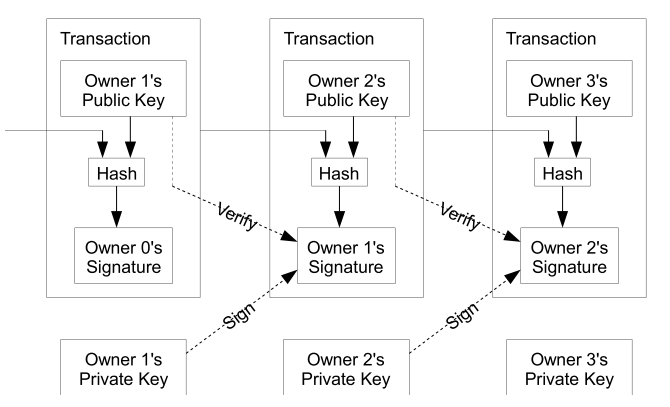
\includegraphics[width=10cm]{transactions.png}
			\centering	
		\end{figure}
		
		The only problem here is that the payee can't prove that the amount the previous owner passed to it was double-spent before the change of ownership. That is, without the full-knowledge of the chronological order of the transactions, a malicious attacker can effectively reuse its money before the payee is able to use it. 
		
		What is needed then is some sort of timestamps service that could put guarantees over the chronological order of the transactions. This is the \textit{trust} that a third party electronic cash system requires for it to work and what such system does is essentially to check that there exists one and only transaction from the sender to the receiver. Furthermore, this means that a system is required to have the \textit{full-knowledge} of its history, meaning that a decentralized system has as a requirement an \textit{agreement} over a single full history of the transactions. Each transaction must be broadcasted among all the nodes of the network.
		
	\subsection{Bitcoin Blockchain}
		The solution that Bitcoin (and the majority of the other cryptocurrencies) adopted to provide the full history of the Bitcoin transaction is to store every user's transaction informations on a public ledger replicated among all the nodes of the network. These information are collected in blocks of transactions and each block refers to its predecessor by including its hash.
		
		\begin{figure}
			\caption{Sketch that shows how the blocks refers with their respective predecessor.}
			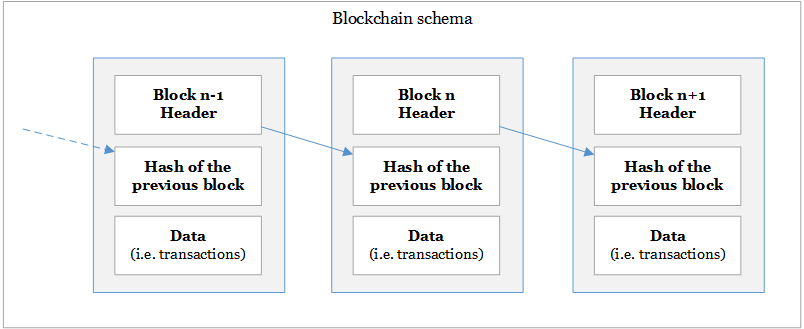
\includegraphics[width=10cm]{blockchain_schema.png}
			\centering	
		\end{figure}
	
		In 2013 C. Decker and R. Wattenhofer \cite{Decker2013} analyzed the behavior of the information propagation in the Bitcoin network and found that the median time for a broadcasted block to reach all the peers is 6.5 seconds (whereas the mean is 12.6 seconds).
		
		What is required then is that the users must all agree on the very same public ledger in order to be sure that a transaction has not been double-spent.
		
	\subsection{Consensus Mechanism}
		The core innovation and the success of the blockchain technology resides in the consensus protocol which will be referred as \textit{Nakamoto Consensus}. Nakamoto Consensus main goal is to reach an agreement over the same public ledger owned by every node of the network, i.e. old blocks and new blocks must be the same for everyone.
		
		The trick here is to use a challenging computational puzzle (that Nakamoto in his paper calls \textit{Proof-of-work}, but it's a misnomer\footnote{Bitcoin's PoW is not a real Proof of Work because it's a probabilistic puzzle, i.e. with a certain luck one is capable to find a solution with very little work. The very first Proof of Work was invented in 1992 by C. Dwork and M. Naor as an anti-spam system \cite{Dwork1992}}) to determine the next block in the chain. Every user can work on the puzzle and try their luck to get the possibility to find a new block.
		
		A block is appended to the head of the blockchain if and only if it is the first to get announced and contains the correct solution to the computational puzzle. Upon hearing the new block, the participant of the network verify that the block is indeed correct, append the block to the head of their blockchain (that is stored locally) and immediately start working on finding the next one.
		
		The computational puzzle is only needed for all nodes to agree on a common value. Because of its random nature, it is likely that only one node will eventually find the solution to such puzzle. Once a block is found, it is propagated through the network. If the solution to the hashing puzzle is valid and if the transactions in the blocks are valid then the block is accepted into the blockchain. A transaction is valid if:
		\begin{enumerate}
			\item each transaction input matches a previous transaction output.
			\item they are reedemed by their legitimate owners
			\item the sum of values of all transaction outputs is less than or equal to the sum of the values of all inputs.
		\end{enumerate}		
		This verification is performed by bitcoin nodes. It would be useless for a malicious user to forge invalid blocks, because any invalid block (malformed blocks, blocks that contain invalid transactions or blocks whose proof-of-work doesn't resolve the puzzle) would be discarded by the honest peers of the network. 
		
		Nakamoto claims that Bitcoin is safe from byzantine failures, as long as 50\% of the total computational power required to solve the cryptographic puzzle belongs to honest miners. If the attackers manage to get more than 50\% of computational power they are more likely to include the block they produced in the blockchain thus making them able to perform devastating strategies that would disrupt the coin (blacklisting particular addresses, coin hostage scenarios...).
		
		It is possible though that two proof-of-work are found within a short time window. This situation is known as a \textit{temporary fork}, a situation in which the blockchain is split in two chains of equal size and was found to happen with a rate of 1,69 every 100 blocks (\(r = 1,69\%\)) (C. Decker, R. Wattenhofer, 2013). Miners will start to produce a block for either one of the two temporary heads of the chain; the random nature of the computational puzzle will eventually extend one of the two forks and sooner or later every node in the network will reach agreement over the longest chain. Resolving a fork is a crucial matter as forks, which theoretically are an inconsistent state of the blockchain, enable a disruptive attack on the network known as \textit{selfish mining} which reduces the computational powers requirements for attackers from 50\% of the total computational power to 33\% \cite{Eyal2013}. Because of this possibility, it has been discovered that Nakamoto suggestion for Byzantine Agreement doesn’t really solve Consensus but solves a weaker version of Consensus in which only agreement is satisfied but validity cannot be guaranteed with overwhelming probability both in synchronous \cite{Garay2015} and in asynchronous settings \cite{Pass2016}.
		
		Although a fork condition happens not so often, it is always advised to wait at least 6 confirmation blocks (roughly one hour) before considering a transaction to be valid.
		
		\subsection{Producing a block}
		
		A node who decides to actively participate by creating new blocks is called \textit{miner}. What a miner does is to gather the maximum number of transactions that can fit in a block (whose size is fixed) and to find a value (\textit{nonce}) that hashes the block and in the meantime whose hash is lesser than a target. More precisely, in order for a block to be valid, the SHA-256 hash of a block's header must be lower to the current \textit{target}, with this last one being a 256-bit number that all the Bitcoin clients share. To increase the possibilities for a transaction to be included in a block, users pay a fee to the miners in proportion to the size of the transaction. As showed in \cite{Gurcan2017}, fairness with respect to the probability for a transaction to be processed is not a guaranteed property as long as the transaction fees are large enough to incentivize a miner to include the transaction in a block.
		
		Finding a block is a cryptographic puzzle, a simple brute force attack on the SHA-256 protocol, whose goal, by picking nonces at random, is to find a hash with \(d\) consecutive zero bits, where \(d\) is called \textit{difficulty} and is derived from the target value in the following way:
		
		\[ d = 8 + \frac{log(D)}{16}\] 
		where
		\[D = \frac{\text{max difficulty}}{\text{target}}\]
		
		The difficulty is calibrated every 2016 blocks (roughly two weeks) so that each solution takes approximately 10 minutes to be found. 
		
		The mining operation requires a lot of computational power and the computational power requires a lot of electrical energy, which in 2014 D. Malone and  K.J. O'Dwyer estimated to be comparable to Ireland's electricity consumption \cite{Malone2014}. That is, producing a block has a high production cost associated. To incentivize the production of new blocks, there's a reward for each miner that can be obtained if and only if a block is successfully added to the blockchain: miners can include a \textit{coinbase} transaction which is capable to generate new coins for the creator of the block; furthermore, this is the only way in which new Bitcoins are input onto the network. Since the coinbase reward is programmed to be halved every 210'000 mined blocks, Nakamoto included transaction fees as another incentive for miners to perform mining.
		
		The incentive also protects the system from attackers: suppose an attacker is able to assemble the majority of the computational power, then he would have to choose between using this power to enable a double-spend attack or to generate new coins. It is much more profitable for him to behave good and play by the rules than to destroy the currency.
		
		\newpage
		
		\subsection{Ownership}
		
		Bitcoin relies on cryptography to allow users to perform operations in a completely secure and private way, making use of \textit{digital signatures} to prove one's identity and \textit{hash function} to verify the integrity of the data in the system.
		There is no concept of "account" in Bitcoin. \textit{Ownership} of the currency means knowledge of the private key that is capable to redeem a certain output. 	Bitcoin transactions express the transfer of value from one \textit{Bitcoin address} to another. A Bitcoin address is the partial hash of a user public keys and it is represented as a string of 26-35 alphanumeric characters.
		
		Each transaction output has a signature validation routine (a script) that verifies the ownership for those that will claim it. This routine is called \textit{scriptPubKey}, also known as "pay-to-pub-key-hash" or P2PKH. It is a script written in the Bitcoin scripting language, a Forth-like, stack language that includes several built-in operations called \textit{opcodes}. 
		
		ECDSA is the protocol used by the Bitcoin network to provide a pair of private and public keys to every user. Every Bitcoin address is the result of the hash of the public portion of the ECDSA private/public key. The amount of Bitcoins that reside in an address can be spent only if a user can prove with his signature that he is the owner of the Bitcoin address. To redeem the coins of an address, the owner proves his identity by inputting the signature and the public key of the \textit{scriptSig} to a \textit{scriptPubKey} of a previous transaction.
		
		Given the following \textit{scriptSig} and \textit{scriptPubKey}:
		
		\begin{verbatim}
		scriptPubKey: OP_DUP OP_HASH160 <pubKeyHash> OP_EQUALVERIFY OP_CHECKSIG
		scriptSig: <sig> <pubKey>
		\end{verbatim}
		
		the script will execute in the following way\footnote{from the Bitcoin wiki. https://en.bitcoin.it/wiki/Transaction\#Pay-to-PubkeyHash}:
		\begin{center}
			\begin{tabulary}{\textwidth}{|L|C|L|}
			\hline
			\textbf{Stack} & \textbf{Script} & \textbf{Description} \\ \hline
			Empty. & <sig><pubKey> OP\_DUP OP\_HASH160 <pubKeyHash> OP\_EQUALVERIFY OP\_CHECKSIG & scriptSig and scriptPubKey are combined. \\ \hline
			<sig> <pubKey> & OP\_DUP OP\_HASH160 <pubKeyHash> OP\_EQUALVERIFY OP\_CHECKSIG & Constants are added to the stack. \\ \hline
			<sig> <pubKey> <pubKey> & OP\_HASH160 <pubKeyHash> OP\_EQUALVERIFY OP\_CHECKSIG & Top stack item is duplicated. \\ \hline
			<sig> <pubKey> <pubHashA> & <pubKeyHash> OP\_EQUALVERIFY OP\_CHECKSIG & Top stack item is hashed. \\ \hline
			<sig> <pubKey> <pubHashA> <pubKeyHash> & OP\_EQUALVERIFY OP\_CHECKSIG & Constant added. \\ \hline
			<sig> <pubKey> & OP\_CHECKSIG & Equality is checked between the top two stack items. \\ \hline
			true & Empty. & Signature is checked for top two stack items. \\
			\hline
			\end{tabulary}
		\end{center}
		
		\subsection{Scaling issue}
		
		Bitcoin has two main limitation that are strongly correlated: throughput of transactions processed and disk space occupied from the blockchain. The correlation is trivial: as long as a block holds more transactions, the throughput increases and the same does the size of the block. Balancing the trade-off is crucial to the cryptocurrency success or failure because either Bitcoin is small in size but is unable then to process more than a few transactions or either it becomes capable to process a great number of transactions while having huge increase in blockchain size. 
		
		The scaling debate as its root since the very first few days of the Bitcoin life: initially set to 1MB per block\footnote{https://github.com/bitcoin/bitcoin/commit/a30b56ebe76ffff9f9cc8a6667186179413c6349\#diff-118fcbaaba162ba17933c7893247df3aR2614}, was later changed to a soft-cap of 250KB for newly created blocks\footnote{https://github.com/bitcoin/bitcoin/commit/c555400ca134991e39d5e3a565fcd2215abe56f6} and later raised up to 750kB\footnote{https://github.com/bitcoin/bitcoin/commit/ad898b40aaf06c1cc7ac12e953805720fc9217c0\#diff-e8db9b851adc2422aadfffca88f14c91R39}. Proposal for a further increase of the maximum block size up to 8MB were made and discussed\footnote{https://github.com/bitcoin/bitcoin/pull/6341}, but were found too risky. Some of these debates resulted in hard-forks, a split that occurs when the underlying protocol changes, thus new \textit{alt-coins} born.
		By the end of the first half of 2015 the blocks were 40\% full. The risk of a saturated network was real, and a number of suggestion came from the Bitcoin developers (as well a proposal for a 4MB block size increase and a 12 seconds latency for each block \cite{Croman}, which are the settings that theoretically maximize the \textit{effective throughput}). 
		
		\section{Micropayments network}
		
		Micropayments are financial transactions of small amounts of money that usually take place on the internet. These payment systems address the problem of transaction fees and processing time, making it easier and cheaper for one user to transfer small amount of funds to another user without incurring in high fees or be slowed down by a financial institutions verifications. There is yet no formal definition for "small amount of money": transaction processors like Visa enable funds transfers from 10\$\footnote{https://usa.visa.com/dam/VCOM/download/merchants/minimum-transactions-credit-card.pdf}, while Paypal and others allow for a minimum of 0.01\$. 
		
		Micropayments system were initially designed in 1960 \cite{Nelson1960}, even before the advent of internet, as a way to pay copyright holders for their fair share. In late 90s there were a lot of attempts on building micropayments networks especially from IBM and Compaq who had their own micropayment division. None of their solutions (along with dozens of others payment system) ever made it to become a micropayment standard. Nowadays the micropayment functionalities is implemented in the most online wallets (PayPal, Swish, Vipps, MobilePay, Postepay) and it is largely implemented in videogames where players can exchange real money with in-game currency in order to purchase virtual goods through in-game micro-transactions. 
		
		The difficulty here for trusted third parties is to keep the processing costs low while keeping available the mediator service in case of disputes and in the same time make earnings over the small transaction with transaction fees. If the burden of mediating disputes can be moved from external agent to payment network users then this would result in near-zero fee for transactions (in digital payments fees are required to prevent dust/flood attacks).
		
		\section{Lightning Network}
		
		In early 2016, J. Poon and T. Dryja released a white paper where a Bitcoin layer 2 decentralized payment system, called Lightning Network, is proposed. The goal of the Lightning Network is to address the scaling problem not on the Bitcoin protocol itself, but by building on top of the Bitcoin system a network of peer-to-peer micro-payment channels where each transactions takes place off-chain.
		
		A micropayment channel is a trustless relationship between two peers of the Bitcoin network, where these two party continuously exchange coins and update their balances, avoiding to broadcast the transaction until both reach an agreement over a final state. This means that almost infinite transactions can occur between two peers without hitting the blockchain (and therefore without incurring in the scaling issues mentioned before), updating the channel balance everytime the two peers wish to perform a transaction and publishing onto the blockchain only the final state agreed by the two users.
		
		 The idea of micropayment channels is not new in the Bitcoin community and it has been around since 2013\cite{Micropayments:Online}\cite{Micropayments:Bitcoinj}. The intuition in Lightning Network was to connect the channels each other in order to allow for those who want to send a payment to any other peer in the network, to ask other users to cooperate in a trustless way to route the payment to the desired receiver.
		
		\subsection{Bi-Directional Payment Channels}
		
		The building block of the Lightning Network are bi-directional payment channels, channels in which a payer sends money to a payee and vice-versa. To build such channels it is required to leverage on the timestamp property of the blockchain and furthermore, a special redeem script is needed along with some particular op-codes. The core ingredients for a bi-directional channels are:
		\begin{itemize}
			\item \textit{2-of-2 Multisignature addresses}: Bitcoin addresses requires to verify two signatures instead of just one (as seen on the scriptPubKey example). An example of real case of 2-of-2 multisignature account are the husband and wife saving accounts where both signatures are required to spend the funds, preventing one spouse from spending without the other spouse's consent. More generally, Bitcoin supports $m$-of-$n$ multisignature addresses meaning that spending from such an address requires m signatures out of n.
			
			\item \textit{Timelocks}: they are a special primitive functions for smart-contracts that prevents outputs from being spent until a specified block heights. Timelocks can either be \textit{absolute} or \textit{relative}:
			\begin{itemize}
				\item absolute timelocks are identified by a special field, nLockTime, that specifies the earliest time (i.e. the block height) a transaction may be added to a valid block. A special op-code, namely OP\_CHECKLOCKTIMEVERIFY\footnote{https://github.com/bitcoin/bips/blob/master/bip-0065.mediawiki} (abbrv. CLTV), allow transactions outputs to be encumbered by the timelock. 
				
				\item relative timelocks are specified by the nSequence fields and allows input to specify the earliest time it can be added to a block based on how long ago the output being spent by that input was included in the blockchain. The OP\_CHECKSEQUENCEVERIFY\footnote{https://github.com/bitcoin/bips/blob/master/bip-0112.mediawiki} provides for relative timelocks the same feature that OP\_CHECKLOCKTIMEVERIFY provides for absolute timelocks.
			\end{itemize}	
			
			\item \textit{SIGHASH\_NOINPUT}: it is a special function of the Bitcoin scripting language that allows dynamic binding of unspent transactions. It modifies the digest algorithm used in the signature creation and verification by removing the dependency on the previous output commitment. With SIGHASH\_NOINPUT\footnote{https://github.com/bitcoin/bips/blob/master/bip-0118.mediawiki\#backward-compatibility} it is possible to have chains of \textit{floating transactions}, i.e. transaction that are not yet published on the blockchain yet related each other.
		\end{itemize}
		
		\subsection{Opening a micro-payment channel}
		
		To open a new bi-directional payment channel, two parties initially must fund the channel with the maximum amount of Bitcoin that they want to be able to spend inside it, by allocating funds on a 2-of-2 multisignature address, i.e. an address that need the cooperation (that is, signatures) of the two parties to be used for further transactions. This is the \textit{Funding Transaction}.
		
		Before signing and broadcasting this transaction, the two party signs and exchange a new transaction called \textit{Commitment Transaction} spending the output of the funding transaction and whose goal is to express the current channel balance. The very first commitment transaction will simply return the money to their legitimate owners: this is done in order to avoid hostage scenarios in which one of the party is uncooperative and it's willing to block any future operation from the funding transaction. For the sake of clarity, say Alice and Bob wants to open a new channel:
		
		\begin{figure}[]
			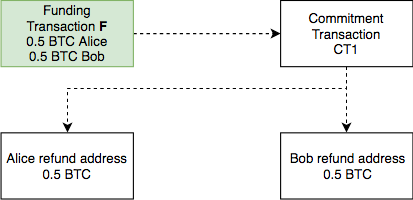
\includegraphics[width=9.5cm, keepaspectratio]{funding}
			\centering
			\caption{The funding transaction is the only one that gets published in the Bitcoin network. The disclosure of CT1 would refund Alice and Bob of their initial input.}
		\end{figure}
		
		\begin{enumerate}
			\item Either one between Alice and Bob make a new funding transaction F allocating funds to a 2-of-2 multisignature address. This transaction is not yet broadcasted in the Bitcoin Network.
			
			\item Alice prepares a commitment transaction CT\textsubscript{1} that spends from F and returns her money back to herself and to Bob. Bob does the same.
			
			\item Alice signs her commitment transaction, CT\textsubscript{A1}, and gives it to Bob. Bob signs his transaction and gives it to Alice (CT\textsubscript{B1}). 
			
			\item Now Alice signs the transaction Bob gave her, CT\textsubscript{AB1}. Bob as well signs the transaction Alice gave him. Now they both have a refund that ensures that they will be able to get back the money from the 2-of-2 address of the funding transaction if the other party is uncooperative.
			
			\item Now it is safe to broadcast the funding transaction onto the blockchain because both Alice and Bob have CT\textsubscript{AB1}, which permit to any of the two to quit the channel anytime they want and get their money back. By the time F gets mined into a block, a channel is opened between Alice and Bob.
		\end{enumerate}
		
		The process is completely asymmetric: every user involved creates its own transaction, signs it and then exchange it with the other user. In the end, Alice and Bob will hold two different transactions, with different transaction IDs, performing the very same operation. Recently a new protocol for the Lightning Network channel update mechanism named \textit{eltoo}\cite{Decker} has been proposed, addressing the asymmetric nature of the process and bringing other improvements on the security of the channels.
		
		Once the opening process is done, the channel is ready for use. The commitment transaction represent the current channel balance, that is the output address in CT\textsubscript{1} are Alice and Bob personal address. In the naive version of this protocol if Alice and Bob wish to update their balance, say Alice wants to give Bob 0.1 BTC, they can simply create a new commitment transaction CT2 where the outputs of CT2 allocates 0.6 BTC to Bob and 0.4 BTC to Alice and rebind the funding transaction outputs to the new commitment transaction input. However, this approach as serious flaws since there is no mechanism that prevents a malicious Alice to restore her previous balance by publishing CT1 before CT2 onto the blockchain, allowing a double-spend attack in a off-chain scenario.
		
		\begin{figure}
			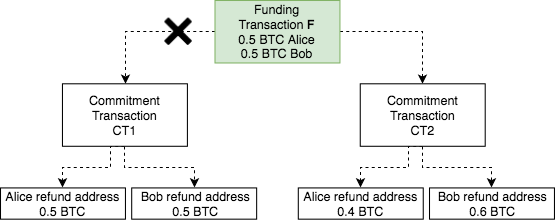
\includegraphics[width=\linewidth]{broken_ct}
			\centering
			\caption{To update the balance, Alice creates a commitment transaction CT2 whose outputs reflect the payment she wishes to perform. In this broken implementation there is no way Bob can react to Alice publishing CT1 after getting paid by her.}
		\end{figure}
		
		\subsection{Fidelity Bonds}
		
		It is necessary then to enforce a condition that prevents older commitment transaction to be broadcast. There are some tools in Bitcoin that let replace a transaction that has yet to be mined with a newer, higher fee transaction\footnote{https://github.com/bitcoin/bips/blob/master/bip-0125.mediawiki}. Yet, in the hypothesis that Bitcoin will be used by billions of people, this on-chain replacement mechanism doesn't scale well because of the scaling issues mentioned before, therefore the revocation of a commitment transaction must be enforced off-chain.
		
		\textit{Fidelity Bonds} are a form of insurance protection against violations of the terms of an agreement, preventing malicious behaviors by any party who adhere to these. The contract terms for a Lightning Network channel is that both the parties involved in the channel agree on the latest commitment transaction. Any attempt on broadcasting an older commitment transaction should result on the loss of all funds in favor of the other party. 
		
		The enforcement of these fidelity bonds are done with the help of two special outputs: \textit{Revocable Sequence Maturity Contract} (abbrv. RSMC) and \textit{Breach Remedy} (abbrv. BR). RSMC are transactions encumbered by the nSequence parameter which is an integer describing how many blocks, starting from parent transaction confirmation, must be waited before the transactions gets mined. Each commitment transaction now has two output: an encumbered refund toward the owner of the CT and an immediate refund output towards the other user in the channel. 
		Figure \ref{rsmc} puts in evidence the user point of views with respect to their floating transaction chain according to the asymmetrical nature of the protocol. If either one of the two party of the channel wishes to broadcast their commitment transaction and redeem the coins then he will be forced by the RSMC to wait a number of confirmation block before being able to get his money back.
		
		\begin{figure}
			\centering
			\begin{subfigure}{0.4\textwidth}
				\centering
				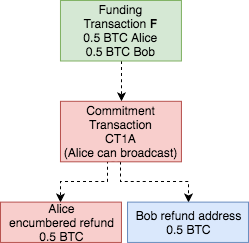
\includegraphics[width=.7\linewidth]{rsmc_a}
				\caption{Alice perspective}
			\end{subfigure}
			\begin{subfigure}{0.4\textwidth}	
				\centering
				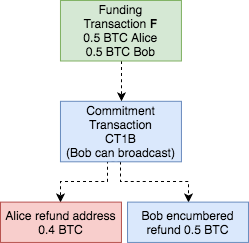
\includegraphics[width=.7\linewidth]{rsmc_b}
				\caption{Bob perspective}
			\end{subfigure}
			\caption{Each user holds different RSMC. Alice can broadcast red transactions, Bob the blue ones. If Alice wishes to broadcast CT\textsubscript{1A}, then she must wait \(n\) confirmation blocks before she can broadcast her refund.}
			\label{rsmc}
		\end{figure}
		
		Encumbering a transaction is required to allow a user to take measures against a misbehavior of the counterpart whenever two users agreed on the latest channel balance. When a new pair of commitment transaction is agreed upon, the previous commitment transaction has to be invalidated. The invalidation routine consists in two new transactions called \textit{Breach Remedy}, that spends from each party old commitment transaction and whose spends transfer all the funds from one user to another whenever an older state is published onto the blockchain. The idea is that by being afraid to commit to such a strong punishment, a user would prefer to just delete old commitment transactions in order to not losing its fund.
		
		\begin{figure}
			\centering
			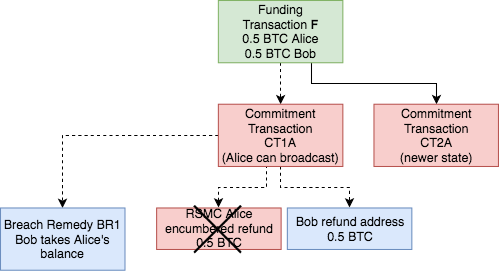
\includegraphics[width=.7\linewidth]{breach_remedy_a}
			\caption{Alice perspective. The encumered RSMC gives Bob time to publish the Breach Remedy and the refund to himself. Alice is encumbered by \textit{nSequence} blocks before she's able to do something.}
		\end{figure}
				
		To close a channel either a commitment transaction is published onto the blockchain, resulting on one of the two party waiting \(n\) blocks before being able to get his money back, or the two agree on the last final state of the balance, namely a \textit{Settlement Transaction}, in which its outputs are not encumbered. Yet it is important to notice that if the two parties remain cooperative, the channel can remain open indeterminately.
		
		\subsection{Hashed Timelock Contracts}
		
		The missing construction that allows to build a network of channel are the \textit{Hashed Time-Lock Contract}, a special contract that allow to maintain a global state across multiple channels based on time commitments (by using the nLockTime parameter) and pre-images discloures.
		The contract is the following:
		\begin{enumerate}
			\item if Bob can produce to Alice within 3 days the input R that hashes to the known hash H, then the contract has to be settled and Alice pays Bob by the sum agreed.
			
			\item after three days without any R disclosure the contract is considered void and the process must be invalidated.
			
			\item the parties involved must payout according to the terms of the contract and close the contract early as soon as both agree.
			
			\item fidelity bonds should occur when the terms of the contract are violated and have to be paid to the non-violating counterparty.
		\end{enumerate}
	
		Essentialy a HTLC is an additional output in the commitment transaction and has two possible spends, where one path is taken if Bob can produce R and the other occurs when a fixed time has passed (we will consider 3 days for further examples). The redeem script is the following:
		\begin{center}
			\begin{tabulary}{\textwidth}{|L|C|}
				\hline
				OP\_IF & \\
				 & OP\_HASH160 <Hash160(R)> OP\_EQUALVERIFY \\
				 & 2 <Alice2><Bob2>OP\_CHECKMULTISIG \\ \hline
				OP\_ELSE & \\
				 & 2 <Alice1><Bob1>OP\_CHECKMULTISIG \\ \hline
				 OP\_ENDIF & \\
				 \hline				 
			\end{tabulary}
		\end{center}
	
		\begin{figure}
			\centering
			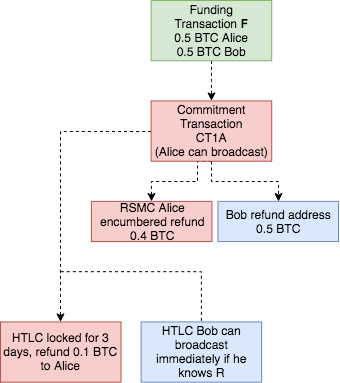
\includegraphics[width=7cm]{htlc_a}
			\caption{Alice perspective. The HTLC represents a pending state in which there is the intent to deliver 0.1 BTC to Bob.}
			\label{htlc_a}
		\end{figure}
	
		If Alice wishes to send 0.1 BTC to Bob by using an HTLC, the two agree on building a new commitment transactions with 3 outputs where the first two are refunds for Alice and Bob (0.4 BTC and 0,5 BTC) while the last one is the 0.1 HTLC pending transaction from Alice to Bob that will either go to Bob if Bob knows R, or refund Alice of its 0.1 BTC in case 3 days elapsed. The invalidation process of an HTLC goes the same as for commitment transaction with HTLC Revocable Sequence Maturity Contract and HTLC Breach Remedy. Once Bob discloses the R, the two can cooperate to update the channel balance in a new commitment transaction in order to maintain the channel open or they could simply push the entire transactions chain onto the blockchain (and thus closing the channel).
		
		\subsection{A Network of Channels}
		
		The use of HTLCs is not intended for a single channel. Instead it is possible now to create a global state across multiple channels, allowing to build the multi-hop payment network that is the Lightning Network. HTLCs allows for time-constrained transactions that force the payee to prove the ownership and oblige the payers to transfer funds before the locktime runs off, in what is known as \textit{chain delegation}, where the burden of the transfer of funds between two users, which don't belong in the same channel, is delegated to the participants of the path that connects the two.

		Let's say Alice wants to pay David and they don't belong in the same channel. Between Alice and David there are Bob and Carol. So Alice can \textit{delegate} Bob to pay David, Bob can do the same with Carol and lastly Carol pays David. With HTLCs these tasks can be set up so that each payment steps can occur before the next is processed in a cascading fashion thanks to the nLockTime parameter. By knowing the number of hops required to reach David, Alice uses that information as the HTLC expiry for its first hop with Bob (say 3 days). Bob will decrement its HTLC expiry by one day with Carol, and Carol will have a 1 day HTLC expiry with David. 
		
		\begin{figure}[h]
			\centering
			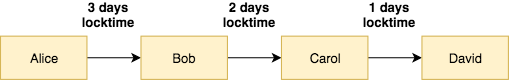
\includegraphics[width=0.7\linewidth]{decrementing_timelocks}
		\end{figure}
	
		In this way the participant will perform their task knowing that the step before has been already performed. Let's say Alice wants to pay David, then David picks a random number R, produces the hash and gives it to Alice. Alice tells Bob that if he can show her R then he will be able to pull funds from her. Bob does the same with Carol and Carol with David. Now on day 1, David knows R so he can pull the funds from Carol. On day 2, Carol shows R to Bob so she can pull funds from Bob and finally on day 3 Bob shows R to Alice, and he's able to pull funds from her as well. Every pair of node settles the new balance with their neighbors in a new commitment transactions and thus the payment is finally over.
		
		Suppose now there are problems between Bob and Carol during the payment, with Bob becoming unresponsive (i.e. broken link). Since Carol cannot settle a new commitment transactions with her updated balance she's forced to publish her chain of floating transaction along with the HTLC of the current operation to the blockchain, eventually disclosing the value of R. By knowing the value of R, Alice can consider the payment done.
		
		Because of their time-dependent nature, nodes and channels are not intended to be considered as static features of a network: a channel can be suddenly closed whenever the locktime runs off, or maybe it is possible that some nodes are inactive during some period of the day (e.g. nodes shutting down during nighttime) so there's the need to capture this property in a model that can describe such dynamic behavior.
		
	\end{document}